\documentclass[a4paper,12pt]{article}

%------------------------- packages -------------------------%
\usepackage[utf8]{inputenc}
\usepackage[T5]{fontenc}
\usepackage[vietnamese]{babel}
\usepackage[unicode,hidelinks]{hyperref}    % for reference
\usepackage{graphicx}
\usepackage{tikz}
\usepackage{amsmath}
\usepackage{geometry}
\usepackage{titlesec}
\usepackage{array}
\usepackage{fancyhdr}  % Ensure this is loaded last
\usepackage{lastpage}
\usepackage{setspace}
\usetikzlibrary{calc}
\usepackage{tabularx}
\usepackage{array}  % For customizing row height
\usepackage{multirow} %dùng cho phần vẽ bảng ở phần lý thuyết
\usepackage[utf8]{inputenc}
\usepackage[utf8]{vietnam}
\usepackage{enumitem}
\usepackage{adjustbox}
\usepackage{amsmath,amsfonts,amssymb}
\usepackage{float}

\usepackage{listings}
\usepackage{tcolorbox}
\usepackage{caption}
\usepackage{listings}
\usepackage{tocloft} % for customizing TOC
% for code and result
\lstset{
  breaklines=true,
  breakatwhitespace=true,
  basicstyle=\ttfamily\small, % Dùng font chữ nhỏ hơn
  columns=fullflexible
}        
        % Khoảng cách từ khung đến nội dung code

\usepackage[svgnames]{xcolor} % Cung cấp nhiều màu sắc hơn
\tcbset{
  colback=AliceBlue,       % Màu nền xanh rất nhạt
  colframe=SteelBlue,      % Màu viền xanh dương đậm
  coltitle=MidnightBlue,   % Màu tiêu đề xanh đen
  coltext=DarkSlateGray,   % Màu chữ chính
  fonttitle=\bfseries      % Font chữ in đậm cho tiêu đề
}


%------------------------- set up -------------------------%
% Set the margins
\geometry{
    left=2cm,
    right=2cm,
    top=2.5cm,
    bottom=2.5cm,
}

%------------------------- header & footer -------------------------%
\renewcommand{\headrulewidth}{0.5pt}
\renewcommand{\footrulewidth}{0.5pt}
\setlength{\headheight}{30pt}
\pagestyle{fancy}

\fancyhead{}    % clear all header fields
\fancyhead[L]{
    \begin{tabular}{ll}
        \begin{picture}(10,10)
            \put(0,-7){
\includegraphics[width=8mm]{hcmut.png}}
        \end{picture}&
        \begin{tabular}{l}
            {\ttfamily Trường Đại học Bách Khoa Tp. Hồ Chí Minh} \\
            {\ttfamily Khoa Khoa học và Kỹ thuật Máy tính} \\
        \end{tabular} 	
    \end{tabular}
}

\fancyfoot{}    % clear all footer fields
\fancyfoot[R]{\footnotesize {\ttfamily Page {\thepage}/\pageref{LastPage}}}

%------------------------- title format settings -------------------------%
\titleformat{\chapter}[display]
  {\normalfont\huge\bfseries}{\chaptertitlename\ \thechapter}{20pt}{\Huge}

% Multi-layered Blue Border Definition
\newcommand{\coverpageborder}{
    \begin{tikzpicture}[remember picture,overlay,inner sep=0,outer sep=0]
        \draw[blue!70!black,line width=4pt] 
            ([xshift=-1.5cm,yshift=-2cm]current page.north east) coordinate (A)--([xshift=1.5cm,yshift=-2cm]current page.north west) coordinate(B)--([xshift=1.5cm,yshift=2cm]current page.south west) coordinate (C)--([xshift=-1.5cm,yshift=2cm]current page.south east) coordinate(D)--cycle;
        \draw ([yshift=0.5cm,xshift=-0.5cm]A)-- ([yshift=0.5cm,xshift=0.5cm]B)--
        ([yshift=-0.5cm,xshift=0.5cm]B) --([yshift=-0.5cm,xshift=-0.5cm]B)--([yshift=0.5cm,xshift=-0.5cm]C)--([yshift=0.5cm,xshift=0.5cm]C)--([yshift=-0.5cm,xshift=0.5cm]C)-- ([yshift=-0.5cm,xshift=-0.5cm]D)--([yshift=0.5cm,xshift=-0.5cm]D)--([yshift=0.5cm,xshift=0.5cm]D)--([yshift=-0.5cm,xshift=0.5cm]A)--([yshift=-0.5cm,xshift=-0.5cm]A)--([yshift=0.5cm,xshift=-0.5cm]A);
        \draw ([yshift=-0.3cm,xshift=0.3cm]A)-- ([yshift=-0.3cm,xshift=-0.3cm]B)--
        ([yshift=0.3cm,xshift=-0.3cm]B) --([yshift=0.3cm,xshift=0.3cm]B)--([yshift=-0.3cm,xshift=0.3cm]C)--([yshift=-0.3cm,xshift=-0.3cm]C)--([yshift=0.3cm,xshift=-0.3cm]C)-- ([yshift=0.3cm,xshift=0.3cm]D)--([yshift=-0.3cm,xshift=0.3cm]D)--([yshift=-0.3cm,xshift=-0.3cm]D)--([yshift=0.3cm,xshift=-0.3cm]A)--([yshift=0.3cm,xshift=0.3cm]A)--([yshift=-0.3cm,xshift=0.3cm]A);
    \end{tikzpicture}
}

%------------------------- tocloft settings -------------------------%
\setlength{\cftbeforesecskip}{0pt} % Space before each section entry
\setlength{\cftsecnumwidth}{2em}   % Width of the section number
\setlength{\cftsubsecindent}{3em}  % Indentation for subsections
\setlength{\cftsubsecnumwidth}{3em}% Width of the subsection number
\setlength{\cftsubsubsecindent}{5em} % Indentation for subsubsections
\setlength{\cftsubsubsecnumwidth}{4em} % Width of the subsubsection number

%------------------------- body -------------------------%

\begin{document}
%-------------------- cover --------------------%
\pagenumbering{gobble}
\begin{titlepage}
    \centering
    
    % Draw the cover page border
    \coverpageborder
    
    % University and Department Info
    \textbf{\large{ĐẠI HỌC QUỐC GIA THÀNH PHỐ HỒ CHÍ MINH}}\\[0.1cm]
    \textbf{\large{TRƯỜNG ĐẠI HỌC BÁCH KHOA}}\\[0.1cm]
    \textbf{\large{KHOA KHOA HỌC VÀ KỸ THUẬT MÁY TÍNH}}\\[0.25cm]
    
    % Logo Positioning
    
\includegraphics[width=0.5\textwidth]{hcmut.png}\\[0.3cm]
    
    % Title and Subtitle
    \textbf{\LARGE{Thiết kế hệ thống AIoT giám sát môi trường thời gian thực trên ESP32}}\\[0.2cm]
    \textbf{\Large{Internet of Things - CO3038}}\\[0.6cm]
    
    % Group Info
    \textbf{\large{LỚP: TN01}}\\[0.2cm]
    \textbf{\large{Giảng viên hướng dẫn: Lê Trọng Nhân}}\\[0.1cm]
    \textbf{\large{\phantom{Giảng viên hướng dẫn:}Phan Văn Sỹ}}
    \begin{table}[h]
    \renewcommand{\arraystretch}{1.5}  % Điều chỉnh chiều cao hàng (1.5 lần bình thường)
    \centering
    \begin{adjustbox}{max width=\textwidth} % Đảm bảo bảng vừa với chiều rộng trang
    \begin{tabular}{|c|l|c|c|c|}
        \hline
        \textbf{STT} & \multicolumn{1}{c|}{\textbf{Họ và tên}} & \textbf{MSSV} & \textbf{Tên lớp} & \textbf{Tên ngành} \\ \hline
        1 & Nguyễn Lưu Khánh Trình & 2313638 & TN01 & Kỹ thuật máy tính \\ \hline
        2 & Trần Minh Trí & 2313626 & TN01 & Kỹ thuật máy tính \\ \hline
    \end{tabular}
    \end{adjustbox}
\end{table}
    
    \vspace{3cm} % Adjust space between the table and the advisor section
   
    
    % Date
    \textbf{\large{THÀNH PHỐ HỒ CHÍ MINH, THÁNG 4 NĂM 2026}}
\end{titlepage}

\clearpage
\pagenumbering{arabic}
\setcounter{page}{1}


%------------------------- re-apply fancy page style -------------------------%
\pagestyle{fancy}

%------------------------- sections -------------------------%

\renewcommand{\contentsname}{Mục lục}
\renewcommand{\listfigurename}{Danh sách hình}
\renewcommand{\listtablename}{Danh sách bảng}

\newpage
\tableofcontents

\newpage
\setstretch{1.25}
\renewcommand{\baselinestretch}{1.25}

%=================== BODY CONTENT ===================%

\newpage
\section*{Abstract}
\addcontentsline{toc}{section}{Abstract}
\textit{[Write a concise abstract: objective, methods, key results, and keywords.]}

\newpage
\section*{Acknowledgement}
\addcontentsline{toc}{section}{Acknowledgement}
\textit{[Write acknowledgements for the instructor, teammates, and useful references.]}

\newpage
\listoffigures

\newpage
\listoftables
\newpage
\section{Introduction}
\subsection{Project Overview}
\textit{This project develops an intelligent IoT system based on the ESP32 platform for real-time environmental monitoring and control. The system collects temperature and humidity data from onboard sensors, presents the readings through a web-based interface, and allows users to configure Wi-Fi settings, track device status, and remotely control selected functions. In addition, the project integrates a Machine Learning/TinyML model to analyze sensor data and provide suitable predictions or recommendations according to the observed environmental state. The proposed solution is designed to support automation, improve the user experience, and remain practical for the limited processing and memory capabilities of the ESP32 microcontroller.}

\subsection{Project Tasks and Requirements}
The implementation is organized into six main tasks:
\begin{enumerate}
	\item \textbf{Task 1: Temperature-driven LED blinking} --- control a status LED blinking pattern according to measured temperature levels.
	\item \textbf{Task 2: Humidity-driven NeoPixel control} --- drive NeoPixel LED color/behavior based on humidity ranges.
	\item \textbf{Task 3: Temperature and humidity monitoring with LCD display} --- read sensor values continuously and show real-time measurements on an LCD interface.
	\item \textbf{Task 4: Web server in Access Point mode} --- deploy an onboard ESP32-S3 web server to provide local configuration and monitoring via AP mode.
	\item \textbf{Task 5: TinyML deployment and accuracy evaluation} --- deploy a TinyML model on-device and assess inference quality through suitable evaluation metrics.
	\item \textbf{Task 6: Data publishing to CoreIoT cloud server} --- transmit collected data and device states to the CoreIoT cloud backend for remote monitoring.
\end{enumerate}

All programming, integration, and testing activities are required to be performed on the \textbf{ESP32-S3} platform using the \textbf{PlatformIO} plug-in as the main development environment.

\subsection{Scope and Limitations}
\textit{[Describe what the report covers and what is outside scope.]}


\subsection{Report Outline}
\textit{[Briefly explain the structure of the remaining chapters.]}


% !TeX root = main.tex
\newpage
\section{Khái niệm hệ thống và cơ sở lý thuyết}
\subsection{Nền tảng IoT}
ESP32 là họ vi điều khiển 32-bit do Espressif Systems phát triển, kế thừa từ ESP8266. Nền tảng này tích hợp kết nối Wi-Fi và Bluetooth/BLE, đồng thời cung cấp hiệu năng xử lý đủ tốt cho các ứng dụng IoT biên. Trong đồ án này, ESP32-S3 được dùng làm bộ điều khiển trung tâm cho các tác vụ cảm biến, xử lý cục bộ, truyền thông và tương tác với đám mây.

\subsubsection{Thông số kỹ thuật chính}
\begin{itemize}
    \item \textbf{Vi xử lý (Processor):} Kiến trúc 32-bit Xtensa/RISC-V (tùy thuộc vào model), thường hoạt động trong dải tần số 160--240 MHz.
    \item \textbf{Bộ nhớ (Memory):} Tài nguyên SRAM tích hợp trên chip với hỗ trợ bộ nhớ Flash ngoài (thông dụng từ 4--16 MB, tùy thuộc vào cấu hình của từng bo mạch).
    \item \textbf{Kết nối (Connectivity):} Hỗ trợ Wi-Fi chuẩn IEEE 802.11 b/g/n và Bluetooth Low Energy (BLE).
    \item \textbf{Giao tiếp ngoại vi (Peripheral Interfaces):} Tích hợp các chuẩn giao tiếp đa dạng như GPIO, PWM, ADC, UART, SPI và I$^2$C.
    \item \textbf{Tính năng quản lý năng lượng (Power Features):} Hỗ trợ các chế độ tiết kiệm năng lượng (low-power modes), phù hợp cho các hệ thống nhúng và thiết bị IoT chạy bằng pin.
    \item \textbf{Điều kiện hoạt động (Operating Range):} Đáp ứng các tiêu chuẩn hoạt động trong môi trường công nghiệp cho các kịch bản triển khai thực tế.
\end{itemize}


\subsubsection{Các tính năng liên quan đến đề tài}
Trong đồ án này, các khả năng sau của ESP32 được sử dụng trực tiếp:
\begin{itemize}
    \item \textbf{Giao tiếp I$^2$C:} Thực hiện kết nối với các cảm biến kỹ thuật số để thu thập dữ liệu nhiệt độ và độ ẩm.
    \item \textbf{GPIO/PWM:} Điều khiển trạng thái đèn LED, cấu hình hành vi của NeoPixel và các cơ cấu chấp hành khác.
    \item \textbf{Hỗ trợ máy chủ Web (Web server support):} Cho phép giám sát và điều khiển thiết bị cục bộ thông qua chế độ Access Point (AP).
    \item \textbf{Hỗ trợ hệ thống tệp trên Flash (ví dụ: LittleFS):} Lưu trữ các tài nguyên web tĩnh (HTML/CSS/JS).
    \item \textbf{Tương thích TinyML:} Khả năng suy luận trực tiếp trên thiết bị để phân tích trạng thái môi trường một cách nhẹ nhàng và tức thời.
\end{itemize}


\subsection{Cơ sở về RTOS}
FreeRTOS là một nhân hệ điều hành thời gian thực (RTOS) gọn nhẹ, mã nguồn mở, được thiết kế cho các hệ thống nhúng có tài nguyên hạn chế. Hệ điều hành này cung cấp một lớp trừu tượng có cấu trúc cho thực thi đồng thời, xử lý sự kiện và đồng bộ giữa các tác vụ mà không yêu cầu lập trình viên phải tự xây dựng cơ chế lập lịch phức tạp. Nhờ chi phí tài nguyên thấp và hệ sinh thái hỗ trợ trưởng thành, FreeRTOS được sử dụng rộng rãi trên các nền tảng vi điều khiển như ESP32, STM32 và ARM Cortex-M.

\subsubsection{Khái niệm cốt lõi}
\begin{itemize}
	\item \textbf{Task (Tác vụ):} là một đơn vị thực thi độc lập, thường được triển khai dưới dạng một vòng lặp vô hạn với không gian bộ nhớ (stack) và trạng thái thực thi riêng.
	\item \textbf{Scheduler (Bộ lập lịch):} thành phần cốt lõi quyết định tác vụ nào được thực thi tại mỗi thời điểm; FreeRTOS thường sử dụng cơ chế lập lịch ưu tiên trưng dụng (preemptive priority-based scheduling).
	\item \textbf{Queue (Hàng đợi):} cơ chế truyền thông an toàn luồng (thread-safe) để truyền tin nhắn hoặc dữ liệu giữa các tác vụ.
	\item \textbf{Semaphore:} một cơ chế đồng bộ hóa được sử dụng để báo hiệu các sự kiện và kiểm soát quyền truy cập vào các tài nguyên dùng chung.
	\item \textbf{Mutex:} một cơ chế khóa chuyên dụng để bảo vệ các tài nguyên dùng chung quan trọng khỏi việc bị truy cập đồng thời.
\end{itemize}


\subsubsection{Vai trò của FreeRTOS trong đồ án}
Trong hệ thống IoT này, FreeRTOS được dùng để điều phối nhiều mô-đun có yêu cầu khắt khe về mặt thời gian và truyền thông:
\begin{enumerate}
	\item \textbf{Quản lý tác vụ đồng thời:} các tác vụ riêng biệt đảm nhiệm việc xử lý web server, lấy mẫu cảm biến định kỳ, thực thi suy luận TinyML và điều khiển LED/thiết bị.
	\item \textbf{Đồng bộ hóa dữ liệu:} semaphore bảo vệ các luồng dữ liệu cảm biến dùng chung, trong khi hàng đợi hỗ trợ việc truyền dữ liệu an toàn giữa các tác vụ.
	\item \textbf{Phản hồi theo mức độ ưu tiên:} tác vụ xử lý yêu cầu web có thể được gán mức ưu tiên cao hơn để đảm bảo khả năng tương tác mượt mà với người dùng; các tác vụ thu thập cảm biến và suy luận được chạy ở mức ưu tiên trung bình một cách có kiểm soát.
	\item \textbf{Cô lập tài nguyên:} mỗi tác vụ có một vùng nhớ (stack) chuyên dụng riêng, giúp giảm thiểu hiện tượng tràn/nhiễu bộ nhớ và cải thiện độ ổn định của toàn hệ thống.
\end{enumerate}

\subsubsection{Kiến trúc tác vụ sử dụng trong đồ án}
Thiết kế phần mềm tuân theo mô hình tổ chức đa tác vụ của FreeRTOS:
\begin{itemize}
	\item \textbf{Task WebServer (mức ưu tiên cao):} xử lý các yêu cầu HTTP và các tương tác trên giao diện người dùng cục bộ.
	\item \textbf{Task Sensor Reader (mức ưu tiên trung bình):} thu thập dữ liệu đo nhiệt độ và độ ẩm định kỳ.
	\item \textbf{Task TinyML (mức ưu tiên trung bình):} thực thi quá trình suy luận trực tiếp trên thiết bị (on-device inference) để dự đoán trạng thái.
	\item \textbf{Task Điều khiển LED/Thiết bị:} cập nhật trạng thái đầu ra của LED/NeoPixel và các cơ cấu chấp hành liên quan.
	\item \textbf{Task Quản lý Wi-Fi:} quản lý kết nối mạng và logic tự động kết nối lại khi mất tín hiệu.
	\item \textbf{Task Nhàn rỗi - Idle Task (mức ưu tiên thấp nhất):} chạy khi không có tác vụ ứng dụng nào sẵn sàng thực thi.
\end{itemize}


\subsection{Cơ sở về TinyML}
TinyML (Tiny Machine Learning) tập trung vào việc triển khai suy luận học máy trên các thiết bị nhúng có tài nguyên hạn chế như vi điều khiển và cảm biến thông minh. Thay vì chuyển luồng dữ liệu cảm biến thô lên máy chủ đám mây để xử lý AI, TinyML thực hiện dự đoán trực tiếp ở biên. Cách tiếp cận này giúp giảm độ trễ, giảm chi phí năng lượng cho truyền thông, tăng cường riêng tư và cho phép hệ thống tiếp tục hoạt động ngay cả khi mạng không ổn định.

\subsubsection{Khái niệm cốt lõi}
\begin{itemize}
    \item \textbf{Suy luận (Inference):} Sử dụng mô hình đã được huấn luyện trước để dự đoán các mẫu dữ liệu đầu vào mới; TinyML chủ yếu tập trung vào quá trình suy luận thay vì huấn luyện trực tiếp trên thiết bị (on-device training).
    \item \textbf{Lượng tử hóa mô hình (Model quantization):} Giảm độ chính xác của các trọng số trong mô hình (ví dụ: từ float32 xuống int8 hoặc int16) nhằm giảm dung lượng bộ nhớ và cải thiện hiệu suất thực thi.
    \item \textbf{TensorFlow Lite / TensorFlow Lite Micro:} Các môi trường thực thi (runtimes) tối giản, được thiết kế để triển khai các mô hình nhỏ gọn trên phần cứng nhúng và thiết bị IoT.
    \item \textbf{Trích xuất đặc trưng (Feature extraction):} Chuyển đổi dữ liệu cảm biến thô thành các đặc trưng có ý nghĩa, phù hợp làm đầu vào cho mô hình.
    \item \textbf{Trí tuệ nhân tạo biên (Edge AI):} Thực hiện các tính toán AI ngay tại nguồn tạo ra dữ liệu (thiết bị biên) thay vì phụ thuộc vào cơ sở hạ tầng đám mây từ xa.
\end{itemize}

\subsubsection{Quy trình phát triển TinyML}
Quy trình triển khai thường bao gồm các bước sau:
\begin{enumerate}
    \item Huấn luyện mô hình ngoại tuyến bằng cách sử dụng các framework học máy trên Python và tập dữ liệu lịch sử.
    \item Chuyển đổi mô hình đã huấn luyện sang định dạng triển khai nhẹ (ví dụ: \texttt{.tflite} hoặc các định dạng biểu diễn nhỏ gọn tương đương).
    \item Áp dụng các kỹ thuật tối ưu hóa và lượng tử hóa để giảm mức sử dụng bộ nhớ và tăng tốc độ thực thi.
    \item Tích hợp các tham số của mô hình vào firmware (ví dụ: dưới dạng tệp tin header của ngôn ngữ C).
    \item Triển khai lên vi điều khiển ESP32-S3 và đánh giá độ trễ thực thi, mức tiêu thụ bộ nhớ cùng chất lượng dự đoán.
\end{enumerate}

\subsubsection{Ứng dụng TinyML trong đồ án}
Trong hệ thống IoT này, TinyML được sử dụng để phân loại trạng thái môi trường từ dữ liệu cảm biến thời gian thực:
\begin{itemize}
    \item \textbf{Đặc trưng đầu vào (Input features):} Nhiệt độ ($^\circ$C) và độ ẩm (\%) thu thập từ cảm biến DHT20.
    \item \textbf{Lớp đầu ra (Output classes):} Các trạng thái hoạt động của môi trường (ví dụ: trạng thái không hợp lệ, chế độ chờ, cần làm mát, cần hút ẩm, cần tạo ẩm).
    \item \textbf{Lựa chọn mô hình:} Thuật toán Naive Bayes với phân phối chuẩn (Gaussian Naive Bayes - GNB), được huấn luyện trên các cặp mẫu nhiệt độ - độ ẩm lịch sử đã được gán nhãn.
    \item \textbf{Tích hợp Firmware:} Các tham số của mô hình được xuất ra tệp \texttt{naive\_bayes\_model.h} và biên dịch cùng với ứng dụng trên ESP32-S3.
\end{itemize}

Để giảm thiểu băng thông giao tiếp, hệ thống có thể chỉ gửi đi các kết quả suy luận ngắn gọn (nhãn trạng thái) thay vì liên tục truyền toàn bộ dữ liệu thô.

\subsection{Cơ sở lý thuyết mô hình Naive Bayes và Phân phối chuẩn (GaussianNB)}

\subsubsection{Định lý Bayes và thuật toán Naive Bayes}
Naive Bayes là một thuật toán phân loại có giám sát dựa trên nền tảng của định lý xác suất Bayes. Mục tiêu của thuật toán là tính toán xác suất để một điểm dữ liệu với vector đặc trưng $X = (x_1, x_2, ..., x_n)$ thuộc về một lớp $y$ cụ thể. Phương trình cốt lõi của định lý Bayes được biểu diễn như sau:

\begin{equation}
P(y|X) = \frac{P(X|y)P(y)}{P(X)}
\end{equation}

Trong đó:
\begin{itemize}
    \item $P(y|X)$ (\textbf{Posterior - Xác suất hậu nghiệm}): Xác suất điểm dữ liệu thuộc lớp $y$ khi đã biết các đặc trưng $X$. Đây là giá trị mô hình cần tối đa hóa.
    \item $P(y)$ (\textbf{Prior - Xác suất tiên nghiệm}): Xác suất xuất hiện của lớp $y$ trong toàn bộ tập dữ liệu, được tính bằng tỷ lệ số mẫu của lớp $y$ trên tổng số mẫu.
    \item $P(X|y)$ (\textbf{Likelihood - Khả năng}): Xác suất quan sát được bộ đặc trưng $X$ nếu điểm dữ liệu thực sự thuộc lớp $y$.
    \item $P(X)$ (\textbf{Evidence - Chứng cứ}): Xác suất xuất hiện của bộ đặc trưng $X$. Do $P(X)$ là hằng số với mọi lớp $y$, ta có thể loại bỏ thành phần này trong quá trình so sánh để tối ưu khối lượng tính toán.
\end{itemize}

Điểm đặc trưng làm nên tên gọi "Naive" (Ngây thơ) của thuật toán là \textit{giả định độc lập có điều kiện} (conditional independence). Thuật toán giả định rằng sự xuất hiện của một đặc trưng $x_i$ hoàn toàn không liên quan đến sự xuất hiện của bất kỳ đặc trưng $x_j$ nào khác khi đã biết lớp $y$. Nhờ giả định này, thành phần Likelihood phức tạp được đơn giản hóa thành tích của các xác suất thành phần:

\begin{equation}
P(X|y) = \prod_{i=1}^{n} P(x_i|y)
\end{equation}

Kết hợp lại, nguyên tắc quyết định phân loại (decision rule) của Naive Bayes là chọn lớp $\hat{y}$ sao cho biểu thức sau đạt giá trị lớn nhất:

\begin{equation}
\hat{y} = \arg\max_{y} \left( P(y) \prod_{i=1}^{n} P(x_i|y) \right)
\label{eq:naive_bayes_base}
\end{equation}

\subsubsection{Biến đổi công thức với Gaussian Naive Bayes (GaussianNB)}
Trong bài toán giám sát môi trường, các đặc trưng đầu vào (Nhiệt độ, Độ ẩm) là các giá trị liên tục (continuous data) thay vì rời rạc (discrete data). Việc đếm tần suất xuất hiện của một con số nhiệt độ chính xác để tính $P(x_i|y)$ là bất khả thi. Để giải quyết vấn đề này, thuật toán \textbf{Gaussian Naive Bayes (GaussianNB)} được áp dụng.

GaussianNB giả định rằng các giá trị liên tục của một đặc trưng trong một lớp nhất định tuân theo \textbf{phân phối chuẩn} (Gaussian Distribution). Thay vì lưu trữ toàn bộ tập dữ liệu, mô hình chỉ cần ước lượng hai tham số thống kê cho mỗi đặc trưng $i$ trong mỗi lớp $y$:
\begin{itemize}
    \item $\mu_{y,i}$: Giá trị trung bình (Mean) của đặc trưng $i$ trong lớp $y$.
    \item $\sigma_{y,i}^2$: Phương sai (Variance) của đặc trưng $i$ trong lớp $y$.
\end{itemize}

Khi đó, thành phần xác suất $P(x_i|y)$ được thay thế bằng hàm mật độ xác suất (Probability Density Function - PDF) của phân phối chuẩn:

\begin{equation}
P(x_i|y) = \frac{1}{\sqrt{2\pi\sigma_{y,i}^2}} \exp\left(-\frac{(x_i - \mu_{y,i})^2}{2\sigma_{y,i}^2}\right)
\label{eq:gaussian_pdf}
\end{equation}

Thay phương trình (\ref{eq:gaussian_pdf}) vào nguyên tắc quyết định (\ref{eq:naive_bayes_base}), ta thu được công thức phân loại hoàn chỉnh của GaussianNB đối với dữ liệu liên tục:

\begin{equation}
\hat{y} = \arg\max_{y} \left( P(y) \prod_{i=1}^{n} \frac{1}{\sqrt{2\pi\sigma_{y,i}^2}} \exp\left(-\frac{(x_i - \mu_{y,i})^2}{2\sigma_{y,i}^2}\right) \right)
\label{eq:gaussian_nb_final}
\end{equation}

Phương trình (\ref{eq:gaussian_nb_final}) chính là nền tảng toán học để huấn luyện mô hình trên Python, từ đó trích xuất các ma trận $\mu$ và $\sigma^2$ nhằm triển khai thuật toán tính toán tối ưu trên vi điều khiển ESP32.

\subsection{Cơ sở về CoreIoT}

\subsubsection{Luồng làm việc trên đám mây và Đường truyền dữ liệu}
CoreIoT là nền tảng quản lý IoT thời gian thực. Hệ thống sử dụng MQTT - giao thức truyền thông Publish/Subscribe hạng nhẹ, đặc biệt tối ưu cho vi điều khiển ESP32. Luồng dữ liệu hai chiều được định tuyến như sau:

\begin{itemize}
    \item \textbf{Chiều lên (Telemetry):} Trạng thái môi trường và thông số ngưỡng được đóng gói thành định dạng JSON, xuất bản (Publish) định kỳ lên đám mây tại topic \texttt{v1/devices/me/telemetry}.
    \item \textbf{Chiều xuống (RPC Control):} Đám mây đóng vai trò Broker điều hướng lệnh điều khiển. ESP32 đăng ký lắng nghe (Subscribe) tại topic \texttt{v1/devices/me/rpc/request/+} để bắt sự kiện từ người dùng và phản hồi xuống phần cứng.
\end{itemize}

\subsubsection{Các thành phần giám sát}
Không gian điều khiển của hệ thống được tích hợp trên Dashboard thông qua hai nhóm thành phần chính:
\begin{itemize}
    \item \textbf{Thành phần hiển thị:} Gồm Thẻ số (Digital Cards) và Biểu đồ đường (Line Charts) để giám sát và lưu trữ chuỗi dữ liệu (time-series) của cảm biến.
    \item \textbf{Thành phần điều khiển:} Gồm thanh trượt (Slider) và công tắc (Switch) liên kết với các phương thức RPC (\texttt{setThre}, \texttt{setStateLED}). Điều này cho phép thay đổi logic điều khiển trực tiếp trên nền tảng Web.
\end{itemize}


\subsection{Tóm tắt chương}
Chương này đã trình bày quá trình thiết kế và triển khai phần mềm cho hệ thống IoT. Nhờ ứng dụng hệ điều hành FreeRTOS, ESP32 đã vận hành trên kiến trúc đa nhiệm gồm: module thu thập dữ liệu (DHT20, LCD), cảnh báo trực quan (LED, NeoPixel), Web Server thiết lập mạng và giao tiếp đám mây CoreIoT qua MQTT. 








\newpage
\section{Thiết kế và triển khai hệ thống}
\subsection{Giới thiệu}
\textit{[Giới thiệu chương triển khai và quy trình thiết kế.]}

\subsection{Nhiệm vụ 1: Nhấp nháy LED theo nhiệt độ}
\textit{[Mô tả logic điều khiển, điều kiện kích hoạt và cách sử dụng semaphore.]}

\subsection{Nhiệm vụ 2: Điều khiển NeoPixel theo độ ẩm}
\textit{[Mô tả mẫu màu, các ngưỡng và cơ chế phối hợp dựa trên semaphore.]}

\subsection{Nhiệm vụ 3: Giám sát nhiệt độ và độ ẩm với LCD}
\textit{[Giải thích việc lấy mẫu cảm biến định kỳ, định dạng dữ liệu và logic cập nhật LCD theo thời gian thực.]}

\subsection{Nhiệm vụ 4: Máy chủ web ở chế độ Access Point}
\textit{[Mô tả thiết lập chế độ AP, thiết kế các HTTP endpoint và xử lý giao diện web trên ESP32-S3.]}

\subsection{Nhiệm vụ 5: Triển khai TinyML và đánh giá độ chính xác}
\textit{[Trình bày luồng tích hợp TinyML, quá trình suy luận trên thiết bị và các thước đo đánh giá.]}

\subsection{Nhiệm vụ 6: Gửi dữ liệu lên máy chủ đám mây CoreIoT}
\textit{[Mô tả định dạng dữ liệu gửi lên đám mây, quy trình publish và chiến lược đảm bảo độ tin cậy/thử lại.]}

\subsubsection{Xây dựng tập dữ liệu}
Đầu tiên, nhóm nghiên cứu thu thập dữ liệu từ cảm biến nhiệt độ và độ ẩm trong môi trường thực tế.
Trong đó file collect\_form\_log.py có nhiệm vụ đọc log cảm biến từ cổng Serial của ESP32 và chuẩn hóa thành tập dữ liệu thô phục vụ huấn luyện. 
Script được thiết kế với cơ chế parse nhiều tầng nhằm tăng khả năng tương thích với các định dạng log khác nhau, bao gồm JSON, chuỗi key-value T/H, và định dạng phân tách bằng dấu phẩy.
Mỗi mẫu hợp lệ được ghi ngay vào CSV kèm timestamp UTC, giúp đảm bảo tính truy vết của dữ liệu. Để tăng độ tin cậy, hệ thống tự khởi tạo header khi file mới, ghi nối dữ liệu ở các phiên thu thập khác nhau, và flush sau mỗi mẫu để hạn chế mất dữ liệu khi dừng đột ngột. 
Kết quả của bước này là tập raw\_data ổn định, làm đầu vào trực tiếp cho khâu gán nhãn và tạo tập train\_ready trong pipeline ML.
Tuy nhiên do nhóm nghiên cứu không thể thu thập data ở trạng thái nhiệt độ, độ ẩm ở mức quá cao hoặc quá thấp nên phải sử dụng các lệnh script khác để tạo thêm dữ liệu đảm bảo tính tổng quát hóa của tập dữ liệu.

Tiếp theo, nhóm tiến hành gán nhãn cho tập dữ liệu thô dựa trên các ngưỡng nhiệt độ và độ ẩm đã định nghĩa. Script extract\_ready\_data.py được phát triển để tự động hóa quá trình này, giúp đảm bảo tính nhất quán và giảm thiểu sai sót so với gán nhãn thủ công.
Quy tắc gán nhán được thiết lập dựa trên các mức nhiệt độ và độ ẩm, ví dụ:
\begin{itemize}
    \item Khi độ ẩm nằm ngoài khoảng [0-100\%] hoặc nhiệt độ nằm ngoài khoảng [-40°C đến 100°C], mẫu được gán nhãn "Không hợp lệ".
    \item  Nhiệt độ 20-30°C và Độ ẩm 30-60
    \item Nhiệt độ > 30°C và Độ ẩm > 60
    \item Các mức khác được gán nhãn tương ứng để tạo ra các lớp phân loại rõ ràng cho mô hình ML.
\end{itemize}
\subsubsection{Huấn luyện các mô hình và đánh giá để chọn mô hình phù hợp nhất}
\textit{[Trình bày các mô hình đã thử nghiệm, tiêu chí đánh giá (độ chính xác, độ trễ, bộ nhớ) và lý do chọn mô hình cuối cùng.]}

\subsubsection{Kiểm thử lại mô hình và nhúng xuống firmware}
\textit{[Mô tả bước kiểm thử sau tối ưu hóa, chuyển đổi mô hình sang định dạng phù hợp (ví dụ: TensorFlow Lite Micro), tích hợp vào firmware và xác minh trên thiết bị thật.]}

\subsection{Tổng quan kiến trúc}
\textit{[Trình bày kiến trúc tổng thể của hệ thống, luồng dữ liệu và sự tương tác giữa các tác vụ.]}

\subsection{Tính mới và cải tiến}
\textit{[Nêu bật các tính năng sáng tạo, nâng cấp giao diện và các mở rộng TinyML để tăng điểm cộng.]}

\subsection{Tóm tắt chương}
\textit{[Tóm tắt nội dung chương triển khai.]}
% !TeX root = main.tex
\newpage
\section{Đánh giá và kết quả thực nghiệm}

\subsection{Kết quả chức năng}
\subsubsection{Task 1 \& 2: LED và NeoPixel}
\begin{figure}[H]
    \centering
    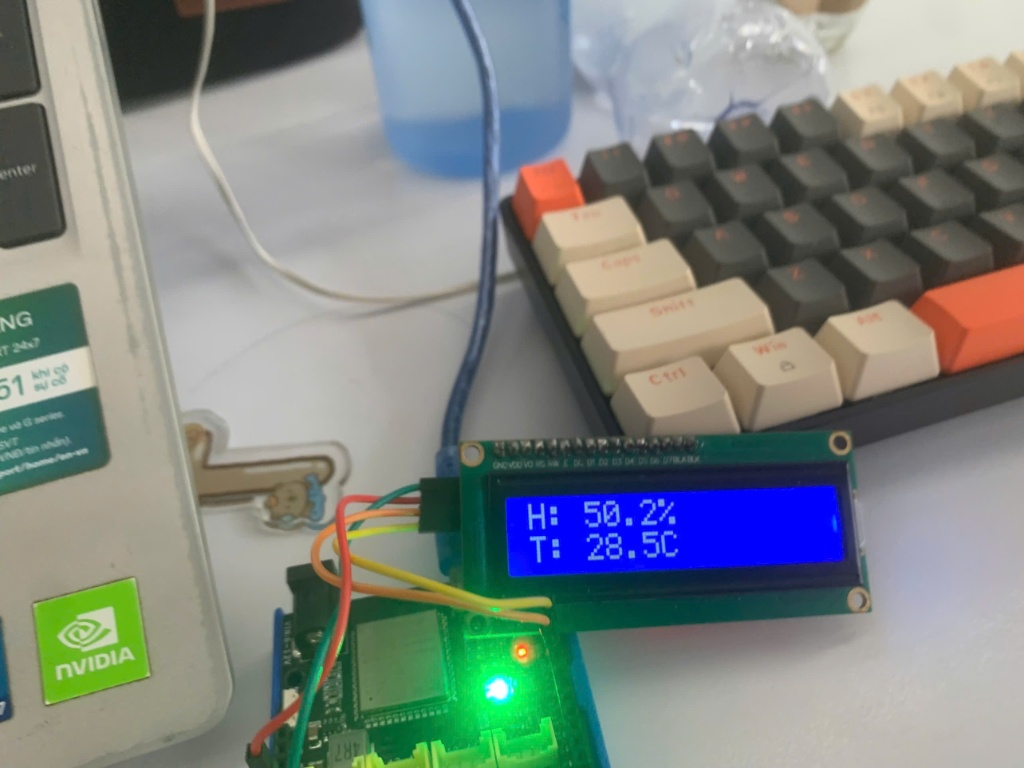
\includegraphics[width=0.75\linewidth]{picture/kq_task_12.png}
    \label{fig:placeholder}
\end{figure}

\begin{itemize}
    \item Led và NeoPixel phản hồi với nhiệt độ độ ẩm đọc từ cảm biến bằng màu sắc 

\end{itemize}

\subsubsection{Task 3: Giám sát môi trường qua LCD}

\begin{itemize}
    \item \textbf{Hiển thị thời gian thực:} Ở chế độ thông thường, màn hình cập nhật chính xác các thông số môi trường 
    \item \textbf{Cơ chế ngắt cảnh báo:} Khi xảy ra sự kiện quá nhiệt (28.4°C > 25°C), màn hình lập tức xóa dữ liệu cũ và thực hiện hiệu ứng chớp tắt dòng chữ \texttt{! WARNING TEMP !} ở hàng trên.
\end{itemize}

\subsubsection{Task 4: Máy chủ Web cục bộ (Local Web Server)}
\begin{figure}[H]
    \centering
    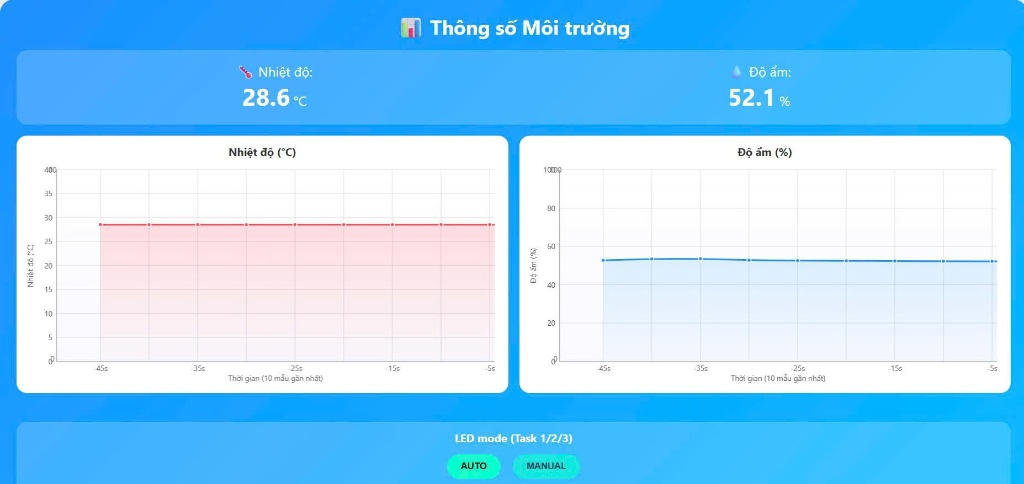
\includegraphics[width=0.75\linewidth]{picture/web_das.png}
    \label{fig:placeholder}
\end{figure}
\begin{figure}[H]
    \centering
    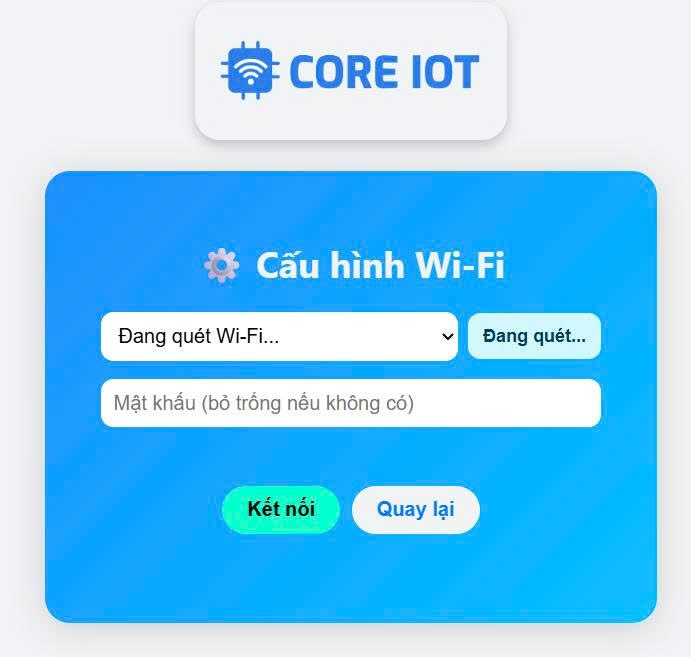
\includegraphics[width=0.75\linewidth]{picture/STA.png}
    \caption{Scan wifi kết nối sang chế độ STA}
    \label{fig:placeholder}
\end{figure}

\begin{figure}[H]
    \centering
    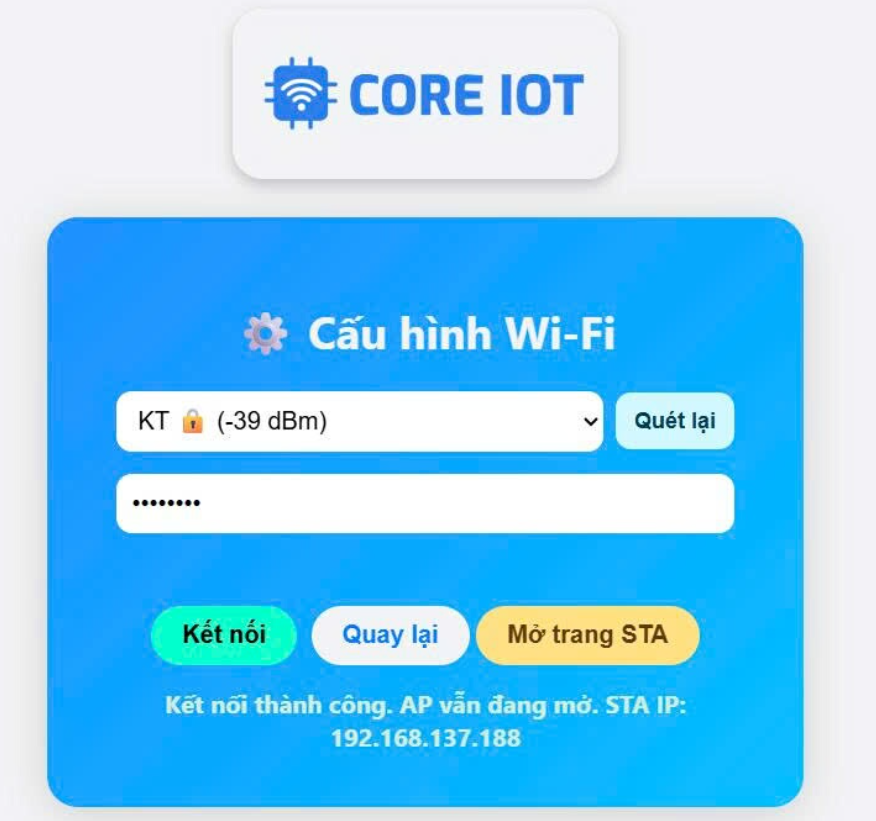
\includegraphics[width=0.6\linewidth]{picture/wifi_connect.png}
    \caption{Sau kết nối wifi thành công}
    \label{fig:placeholder}
\end{figure}

\begin{itemize}
    \item \textbf{Cấu hình mạng (AP Mode):} Cung cấp giao diện "Cấu hình Wi-Fi" , cho phép người dùng quét và nhập mật khẩu kết nối mạng nội bộ. Sau khi kết nối thành công với wifi sẽ cung một địa chỉ IP mới ở chế độ STA.
    \item \textbf{Giám sát nội bộ (SPA Dashboard):} Giao diện Web hiển thị số liệu trực quan với biểu đồ thời gian thực cho cả Nhiệt độ  và Độ ẩm. Các khối chức năng điều khiển chế độ LED (AUTO/MANUAL) và tinh chỉnh màu sắc đều hiển thị.
\end{itemize}

\subsubsection{Task 5: (TinyML)}
\begin{figure}[H]
    \centering
    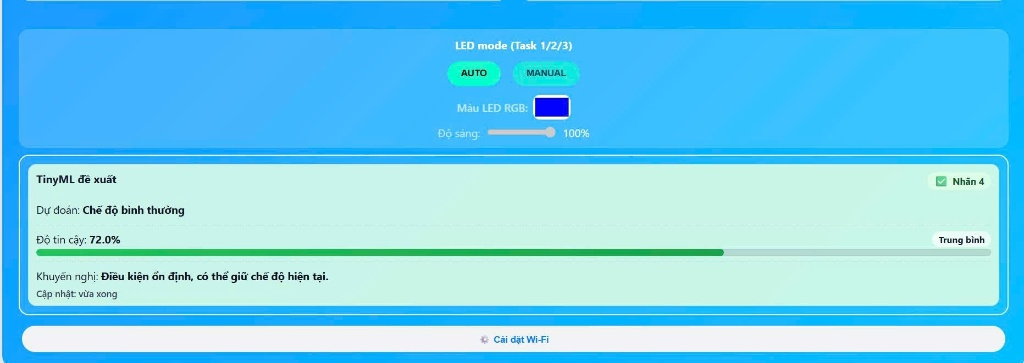
\includegraphics[width=0.75\linewidth]{picture/ml.png}
    \label{fig:placeholder}
\end{figure}




Thuật toán Naive Bayes được nhúng thành công và có khả năng đưa ra các suy diễn logic ngay trên phần cứng hạn chế của ESP32:
\begin{itemize}
    \item Thông qua giao diện Web, hệ thống trả về kết quả dự đoán "Chế độ bình thường" (Nhãn 4) với độ tin cậy (Confidence) đạt 72.0%.
    \item Dựa trên kết quả này, hệ thống chủ động đưa ra khuyến nghị: "Điều kiện ổn định, có thể giữ chế độ hiện tại". Điều này chứng minh tính thực tiễn của Edge AI trong việc hỗ trợ ra quyết định.
\end{itemize}

\subsubsection{Task 6: Tích hợp đám mây CoreIoT}
\begin{figure}[H]
    \centering
    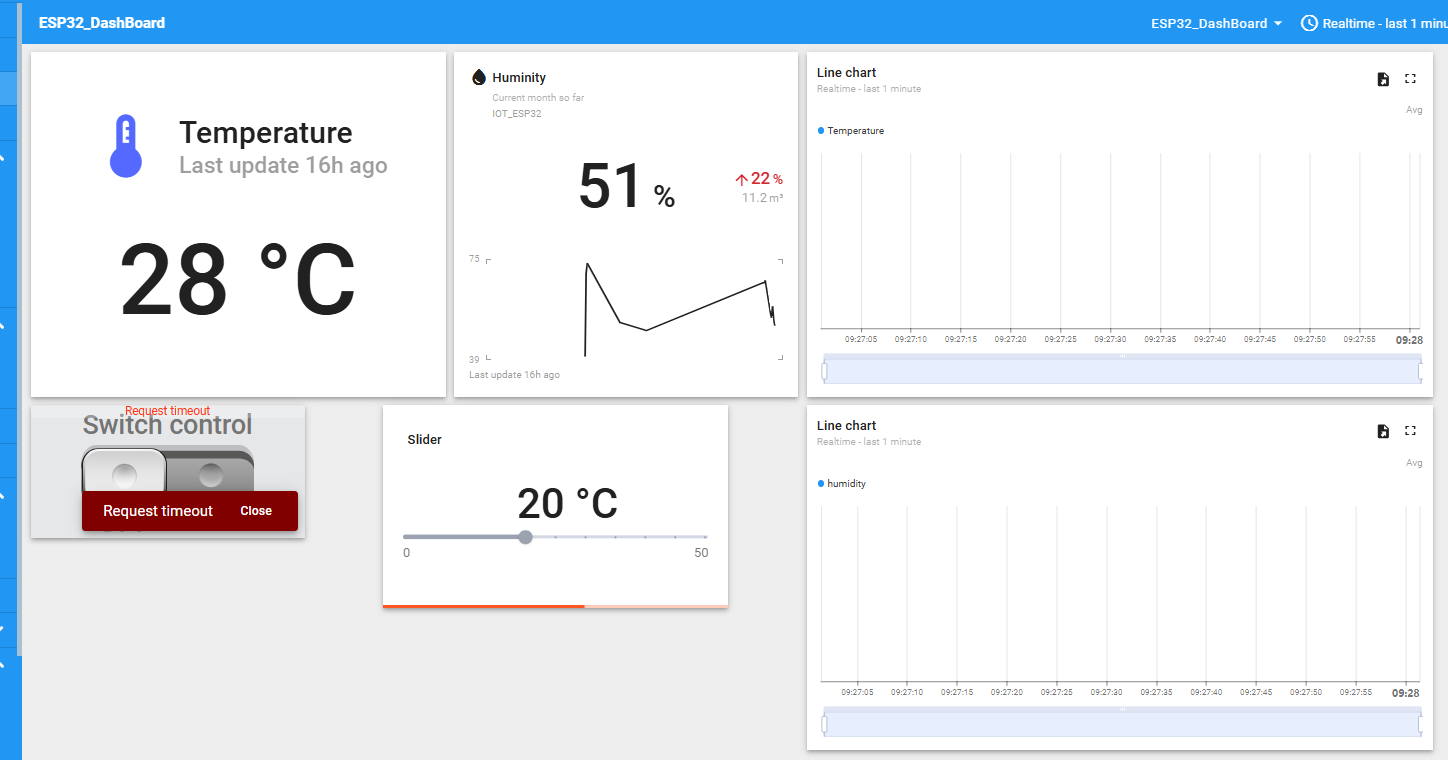
\includegraphics[width=0.75\linewidth]{picture/coreiot.png}
    \caption{Cấu hình ngưỡng nhiệt độ trên CoreIot}
    \label{fig:placeholder}
\end{figure}


\begin{figure}[H]
    \centering
    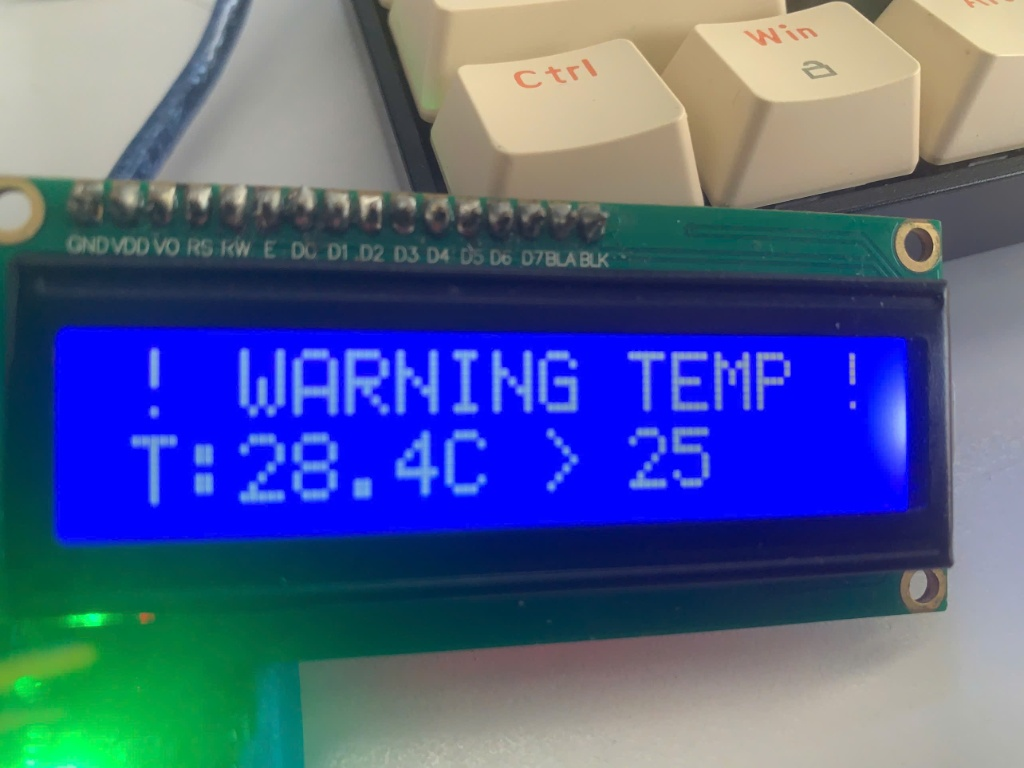
\includegraphics[width=0.75\linewidth]{picture/warning.png}
    \caption{Phản hồi thiết bị với ngưỡng nhiệt độ mới}
    \label{fig:placeholder}
\end{figure}


\begin{itemize}
    \item \textbf{Đồng bộ  (Telemetry):} Dashboard trên ThingsBoard nhận và trực quan hóa dữ liệu ổn định 
    \item \textbf{Điều khiển RPC và Xử lý ngoại lệ:} Thanh Slider thiết lập ngưỡng nhiệt độ (setThre) hoạt động  (ang ở mức 20°C.
\end{itemize}



\subsection{Tóm tắt chương}

Chương này đã trình bày các kết quả kiểm thử và đánh giá của hệ thống sau khi hoàn thiện. Ở phần kết quả chức năng, các chức năng chính của hệ thống đã được kiểm tra để xác nhận tính ổn định, khả năng hoạt động đúng theo yêu cầu và mức độ đáp ứng trong thực tế. Bên cạnh đó, phần đánh giá TinyML cho thấy mô hình có thể được triển khai hiệu quả trên thiết bị biên với tài nguyên hạn chế, đồng thời vẫn bảo đảm được sự cân bằng giữa độ chính xác, dung lượng bộ nhớ sử dụng và tốc độ suy luận. Từ các kết quả đạt được, có thể khẳng định giải pháp đề xuất phù hợp với định hướng ứng dụng IoT kết hợp AI nhúng và có tính khả thi khi triển khai thực tế.



\newpage
\section{Conclusions and Group Discussion}
\subsection{Discussion and Conclusions}
\textit{[Reflect on the implementation process, challenges, lessons learned, and final conclusions.]}

\subsection{Future Perspectives}
\textit{[Suggest future improvements or a reimplementation approach, for example MicroPython.]}
\newpage
\section*{Bibliography}
\addcontentsline{toc}{section}{Bibliography}
\begin{thebibliography}{99}
\bibitem{ref1} [Add reference 1]
\bibitem{ref2} [Add reference 2]
\end{thebibliography}
% !TeX root = main.tex
\newpage
\appendix
\section{Phụ lục A: Tổ chức nhóm}
\textit{[Bổ sung vai trò từng thành viên, trách nhiệm và thông tin đóng góp Git tại đây.]}

\newpage
\section{Phụ lục B: Tài liệu bổ sung}
\textit{[Bổ sung sơ đồ khối, trích đoạn mã nguồn và các kết quả phụ trợ tại đây.]}

\end{document}






